\section{Introduction}
\label{sec:introduction}
% state the learning objective 
The objective of this laboratory assignment is to study a circuit containing a
AC voltage source $v_s$, seven resistors, a voltage-controlled current source $I_b$, a capacitor $C$
and a current-controlled voltage source $V_d$. The components of this circuit are distribuited 
by 4 elementary meshes and 8 nodes, as seen in Figure~\ref{fig:circuit}. 

In order to analyse the circuit, the following data were obtained by running the supplied Python script: 

\textit{Units for the values:} V, mA, uF, kOhm and mS\par
\textit{Values:}


 

R1 = 1.00147062639\par
R2 = 2.0078068512\par
R3 = 3.11269704405\par
R4 = 4.10609573471\par
R5 = 3.02670672634\par
R6 = 2.01292455078\par
R7 = 1.02905244808\par
Vs = 5.24842063411\par
C = 1.04086013403\par
Kb = 7.21413591579\par
Kd = 8.01455113996


In Section~\ref{sec:analysis}, a theoretical analysis of the circuit, 
performed on Octave, is presented. In Section~\ref{sec:simulation}, the 
circuit is analysed by simulation, using NGSpice, and the results are compared to 
the theoretical results obtained in Section~\ref{sec:analysis}. The conclusions 
of this study are outlined in Section~\ref{sec:conclusion}.

\begin{figure}[H] \centering
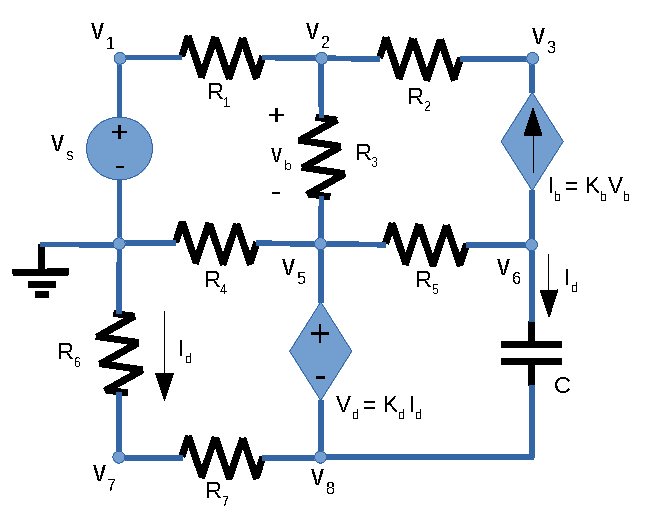
\includegraphics[width=0.4\linewidth]{circuit.pdf}
\caption{Circuit which will be analysed during this laboratory assignment.}
\label{fig:circuit}
\end{figure}

